\section{FFT of an almost Periodic Signal}
\label{almostPeriod} 
In section \ref{FFT_Lines_Beams} we have seen the Fourier transform of an image with equally spaced lines. This is a periodic pattern. But what happens if the pattern is not completely periodic anymore? By taking out one of the lines we explore the effect on the Fourier transform. In figure \ref{fig:fft_lines_almostper} we see the image, where the line which should be at $x=90$ is missing. From figure \ref{fig:fft_lines_cut_almostper} we see that the frequency spectrum still has the same shape, but the intensity range changes. The background which before was at zero (in order to plot logarithmic we added a small value) is now lifted to an intensity of $100$. 
\begin{figure}[H]
	\centering
		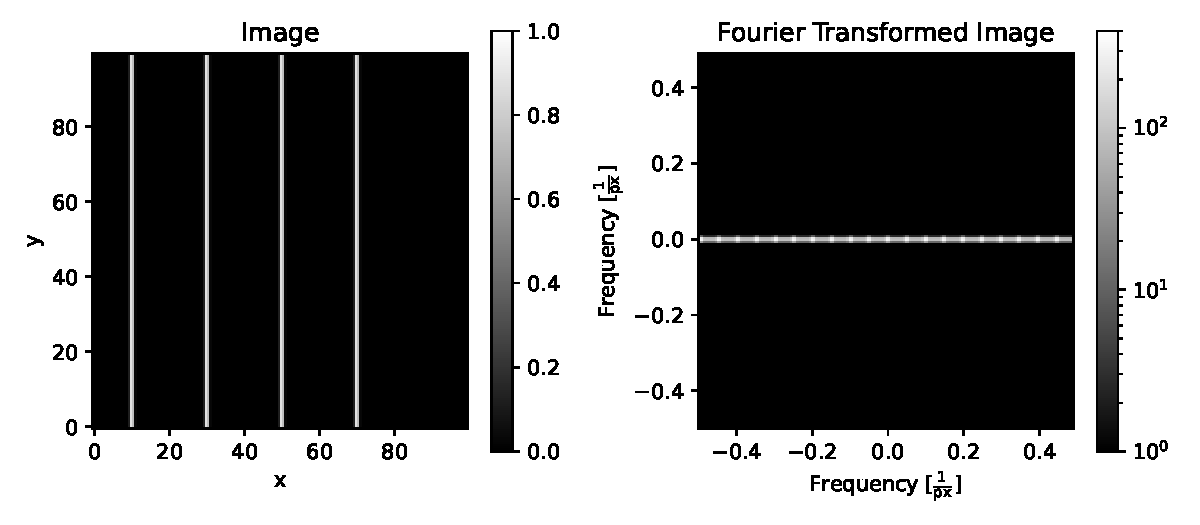
\includegraphics[width=1.0\textwidth]{pics/fft_simulationmorelines_almostper.pdf}
		\caption{An image with several one pixel thick lines which are almost periodically distributed on the left is transformed to the frequency plane, see image on the right.}
		\label{fig:fft_lines_almostper}
\end{figure}
\begin{figure}[H]
	\centering
		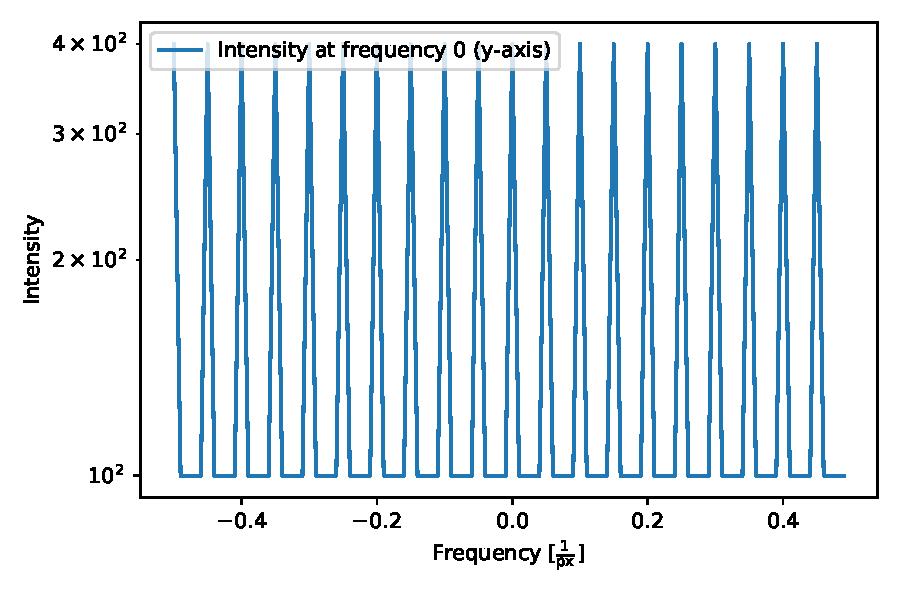
\includegraphics[width=0.8\textwidth]{pics/fft_simulation_cutmorelines_almostper.pdf}
		\caption{The intensity of the Fourier transformed image in figure \ref{fig:fft_lines_almostper} at y frequency zero.}
		\label{fig:fft_lines_cut_almostper}
\end{figure}